\chapter{ಇದೇ ಮಾಯಾ ಚೌಕ}

ಈ ಕೆಳಗೆ ಕೊಟ್ಟಿರುವ ಚಿತ್ರ ಗಮನಿಸಿ. ನಿಮಗೇನು ಅನ್ನಿಸುತ್ತದೆ ?
\begin{figure}[H]
  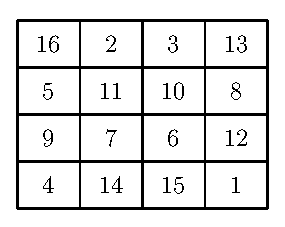
\includegraphics{src/figures/chap1/fig1-1.eps}
\end{figure}
ಇದೊಂದು 16 ಮನೆಯ ಚೌಕ. ಅದರೊಳಗೆ ಸಂಖ್ಯೆಗಳನ್ನು ತುಂಬಿಸಿದೆ. ಯಾರುಬೇಕಾದರೂ, ಎಷ್ಟು ಬೇಕಾದರೂ ಇಂತಹುದನ್ನು ರಚಿಸಬಹುದು ಎನಿಸುತ್ತದೆಯಲ್ಲವೇ?

ಹಾಗಾದರೆ ಈಗ ನೋಡಿ ಇದರ ವಿಶೇಷತೆಗಳನ್ನು ಹಾಗೂ ವೈಚಿತ್ರ್ಯವನ್ನು ಮೇಲಿನ ಅಡ್ಡಸಾಲಿನ ಸಂಖ್ಯೆಗಳನ್ನು ಕೂಡಿಸಿ.

$16+2+3+13=34$
ಇದೇ ರೀತಿ ಬೇರೆ ಅಡ್ಡಸಾಲುಗಳ ಸಂಖ್ಯೆಗಳ ಮೊತ್ತ ಬರೆಯಿರಿ.

\begin{align*}
5+11+10+8 & = 34\\
9+7+6+12 & = 34\\
4+14+15+1 & = 34
\end{align*}
ಇಷ್ಟೇ ಅಲ್ಲ. ಕಂಭ ಸಾಲುಗಳ ಸಂಖ್ಯೆಗಳ ಮೊತ್ತ ಬರೆಯಿರಿ.

\begin{center}
\begin{tabular}{rrrr}
16 & 2 & 3 & 13 \\
5 & 11 & 10 & 8\\
9 & 7 & 6 & 12\\
4 & 14 & 15 & 1\\
34 & 34 & 34 & 34 
\end{tabular}
\end{center}

ಈ ಚೌಕದಲ್ಲಿ ಹೊಸತೇನೋ ಕಂಡು ಬರುತ್ತದೆಯಲ್ಲವೇ? ಇನ್ನೂ ಇದೆ ಇದರ ಲಕ್ಷಣಗಳು. ನಾಲ್ಕು ಮೂಲೆಗಳ ಸಂಖ್ಯೆಗಳ ಒಟ್ಟು ಎಷ್ಟು ನೋಡಿ.

ಹಾಗೆಯೇ ಮಧ್ಯದ ನಾಲ್ಕು ಸಂಖ್ಯೆಗಳನ್ನು ಕೂಡಿಸಿ ನೋಡಿ.

$11+10+7+6 = 34$

ಮೊದಲ ಮತ್ತು ಕೊನೆಯ ಅಡ್ಡಸಾಲು ಹಾಗೂ ಕಂಭ ಸಾಲುಗಳಲ್ಲಿನ ಅಂಚಿನ ಸಂಖ್ಯೆಗಳ ಮೊತ್ತ ನೋಡೋಣ.

$2+3+14+15 = 34$

$5+9+8+12 = 34$

\noindent 
ಕರ್ಣ ಸಾಲುಗಳ ಅಂದರೆ ಮೂಲೆಯಿಂದ ಮೂಲೆಗೆ ಇರುವ ಸಂಖ್ಯೆಗಳ ಒಟ್ಟನ್ನು ಪರಿಶೀಲಿಸಿ.

$16+11+6+1 = 34$

$13+10+7+4 = 34$

ಮುಂದುವರೆದಂತೆ ಚೌಕವನ್ನು ನಾಲ್ಕು ಸಮಭಾಗ ಮಾಡಿ. ಪ್ರತಿಭಾಗದಲ್ಲಿನ ನಾಲ್ಕು ಸಂಖ್ಯೆಗಳ ಮೊತ್ತ ಗಮನಿಸಿ.
\begin{figure}[H]
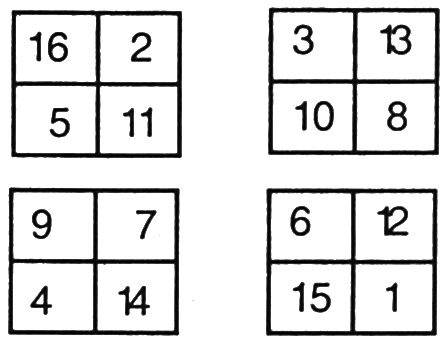
\includegraphics{src/figures/chap1/fig1-2.jpg}
\end{figure}
ಎಲ್ಲ ನಾಲ್ಕು ಚೌಕಗಳಲ್ಲಿನ ಸಂಖ್ಯೆಗಳನ್ನು ಕೂಡಿಸಿದರೆ, ಪ್ರತಿಯೊಂದೂ $34$ ಆಗುತ್ತದೆ.

ಇನ್ನೂ ಕೆಲವು ಕುತೂಹಲಕಾರಿ ಅಂಶಗಳು ಈ ಚೌಕದಲ್ಲಿವೆ. ಅವುಗಳನ್ನು ಮುಂದೆ ತಿಳಿಯೋಣ.

ಈಗ ಹೇಳಿ, ಯಾರು ಬೇಕಾದರೂ, ಎಷ್ಟು ಬೇಕಾದರೂ ಇಂತಹ ಚೌಕಗಳನ್ನು ರಚಿಸಬಹುದೇ ? ಇಲ್ಲ ಎನ್ನುವಿರಾ ? ಅಲ್ಲ, ಸಾಧ್ಯ. ಇದರ ನಿಯಮ, ಸೂತ್ರ, ವಿಧಾನಗಳನ್ನು ಅಧ್ಯಯನ ಮಾಡಿದರೆ ಯಾರೂ ಇಂತಹ ಚೌಕಗಳನ್ನು ರಚಿಸಬಹುದು.

ಈ ಚೌಕಗಳಿಗೆ ಗಣಿತಶಾಸ್ತ್ರದಲ್ಲಿ ‘‘ಮಾಯಾಚೌಕ’’ (Magic Square) ಎಂಬ ಹೆಸರಿದೆ. ಮಾಯಾಚೌಕಗಳು ಎಂದು ಮೊದಲಿಗೆ ರಚಿಸಲ್ಪಟ್ಟವು. ಯಾವಾಗ ಮತ್ತು ಯಾವ ಪ್ರದೇಶದಲ್ಲಿ ಎನ್ನುವುದನ್ನು ತಿಳಿಯಬೇಕೆ ? ಈ ಗ್ರಂಥದ ಕೊನೆಯ ಭಾಗದಲ್ಲಿರುವ 1ನೇ ಅನುಬಂಧವನ್ನು ಓದಿ.
